\chapter{System-level Design}
\label{chap:system-level-design}

\section{Product architecture}


\section{Sub-systems}

\subsection{Data collection}

% - 12 hour monitoring (12:00 - 24:00)
% - Footage stored on internal SD card
% - 4 cameras (Reolink RLC-520A)
% - PoE cameras (powered by single PoE switch)
% - Mounted with 3d-printed brackets
% - on top of tall infrastructure or with aluminum poles where needed
% - placed at entrance and exit points
% - placed to capture full entrance/exit width
% - important in order to be able to calculate ingress/egress (later section)
% -


Data collection is the vital first step in the system, as it provides the raw data needed for all subsequent processing and analysis. This process involved on-site deployment of designated cameras, strategically positioned to capture the crowd dynamics of interest.

The selected cameras were Reolink RLC-520A, which are PoE-enabled (Power over Ethernet) and capable of recording 5MP (2560x1920 pixels) video at 30 frames per second. Powering the cameras required a separate PoE switch (Ubiquiti PoE++ Adapter), which was connected to a standard power outlet. Mounting the cameras was achieved with 3D-printed brackets, designed to securely attach the cameras to existing infrastructure, such as fences or poles. In cases where existing structures were not available, aluminum poles were brought to provide sufficient height in order for the cameras to capture the entirety of the desired area.

As agreed upon with Roskilde Festival's safety team, the cameras were installed around the Eos stage during the first three days of the festival, and subsequently moved to the Arena stage for the remainder of the festival.

\begin{figure}[H]
  \centering
  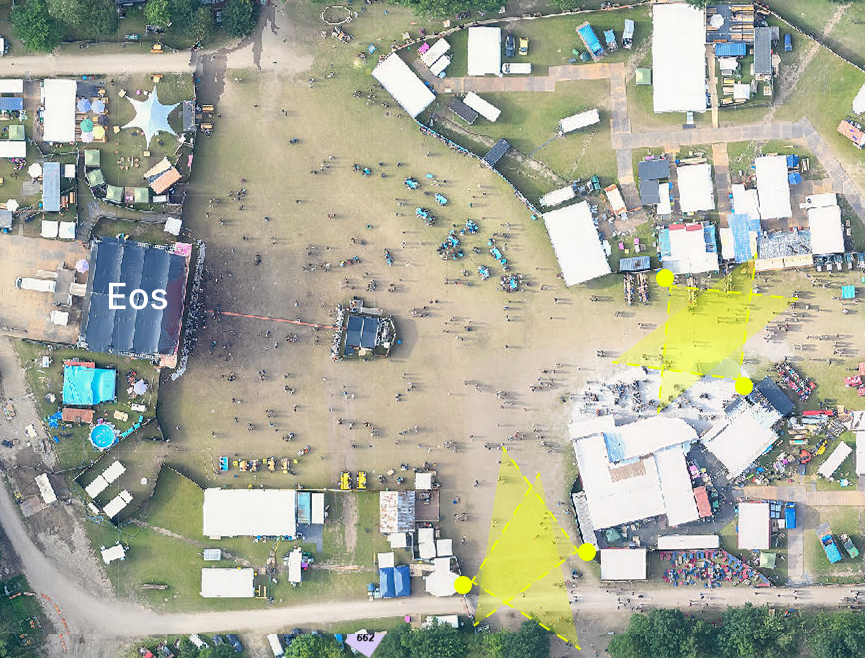
\includegraphics[width=0.9\textwidth]{Pictures/Figures/eos_cameras.png}
  \caption{Camera placement at Eos stage, with approximate field of view (FOV) indicated.}
  \label{fig:eos_cameras}
\end{figure}

\begin{figure}[H]
  \centering
  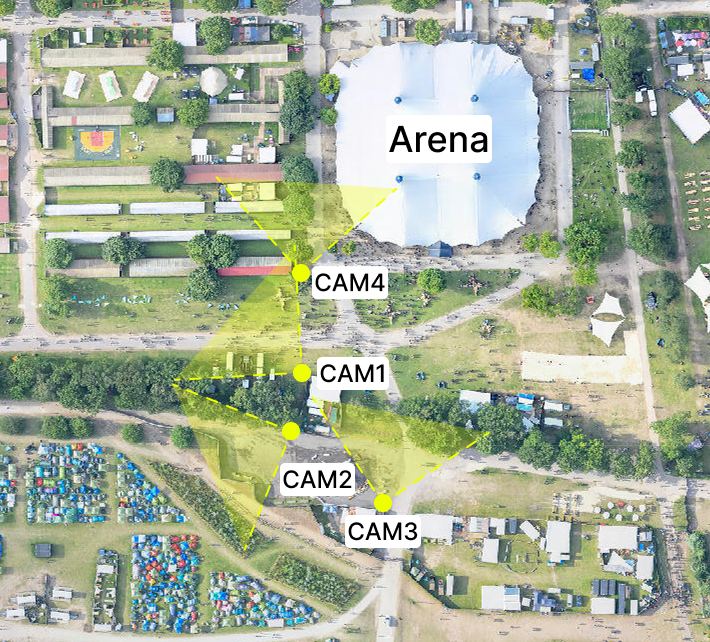
\includegraphics[width=0.8\textwidth]{Pictures/Figures/arena_cameras.png}
  \caption{Camera placement at Arena stage, with approximate field of view (FOV) indicated.}
  \label{fig:arena_cameras}
\end{figure}




\subsection{Computer vision model}

\subsubsection{Annotation}

\subsection{Spatial mapping and GIS}

\subsection{Metric extraction}

\subsection{Interface/frontend}
